\documentclass[11pt, oneside]{article}
\usepackage[letterpaper, margin=2cm]{geometry}
\usepackage{MATH566}
%\usepackage{sagetex}

\begin{document}
\noindent \textbf{\Large{Caleb Logemann \\
MATH 566 Discrete Optimization\\
Homework 3
}}

%\lstinputlisting[language=Sage]{03_2.sage}
\begin{enumerate}
    \item % #1
        Show that
        \begin{center}
            $A\v{x} = \v{b}$ has a nonnegative solution iff
            $\forall \v{y} \in \RR^m$ with $\v{y}^T A \ge \v{0}^T$ implies
            $\v{y}^T \v{b} \ge 0$
        \end{center}
        implies
        \begin{center}
            $A\v{x} \le \v{b}$ has a nonnegative solution iff
            $\forall \v{y} \in \RR^m$, $\v{y} \ge \v{0}$ with $\v{y}^T A \ge \v{0}^T$
            implies $\v{y}^T \v{b} \ge 0$.
        \end{center}

        \begin{proof}
            First let me rewrite the original theorem in different notation for
            clarity.
            Let $C \in \RR^{m \times q}$ and$\v{d} \in \RR^m$, then
            $C\v{u} = \v{d}$ has a nonnegative solution if and only if for all
            $\v{v} \in \RR^m$ with $\v{v}^T C \ge \v{0}^T$ then
            $\v{v}^T \v{d} \ge 0$.
            
            Consider the matrix inequality $A\v{x} \le \v{b}$ for
            $A \in \RR{m \times n}$ and $\v{b} \in \RR^m$.
            Let $\v{z} = \v{b} - A\v{x}$

            First let $A\v{x} \le \v{b}$ have a nonnegative solution, that is
            there exists $\v{x} >= \v{0}$ such that $A\v{x} \le \v{b}$.
            Let $\v{y} \in \RR^m$, with $\v{y} \ge \v{0}$ and $\v{y}^T A \ge \v{0}^T$.
            If we right multiply by $\v{x}$, we see that $\v{y}^T A\v{x} \ge 0$.
            Since $\v{y} \ge \v{0}$ and $\v{b} \ge A\v{x}$, we know that
            $\v{y}^T \v{b} \ge \v{y}^T A\v{x} \ge 0$.
            Thus $\v{y}^T \v{b} \ge 0$.

            Second assume that if for all $\v{y} \in \RR^m$ such that
            $\v{y} \ge \v{0}$ and $\v{y}^T A \ge \v{0}^T$ then
            $\v{y}^T \v{b} \ge 0$.

        \end{proof}

    \item % #2 Done
        Some university in Iowa was measuring the loudness of the fan's
        screaming during the first touchdown of the local team.
        The measurements contain loudness in dB and the number of people at the
        stadium in thousands
        \begin{center}
            \begin{tabular}{*{6}c}
                \toprule
                \# fans & 53 & 55 & 59 & 61.5 & 61.5 \\
                \midrule
                dB     & 90 & 94 & 95 &  100 &  105 \\
                \bottomrule
            \end{tabular}
        \end{center}
        Find a line $y = ax + b$ best fitting the data.
        There are several different notions of best fitting.
        Commonly used is least squares that is minimizing $\sum*{i}{}{\p{ax_i + b - y_i}^2}$.
        But big outliers move the result a lot (and it is troublesome to do it
        using linear programming).
        Use the one that minimizes the sum of differences. That is
        \[
            \sum*{i}{}{\abs{a x_i + b - y_i}}
        \]
        Write a linear program that solves the problem and solve if for the
        ``measured'' data.

        The linear program's objective function should minimize the sum of the
        absolute values of the errors.
        However a linear program's objective function must be linear and
        therefore can't contain any absolute values funtions.
        Instead let $\abs{a x_i + b - y_i} \le e_i$.
        When $\sum*{i}{}{e_i}$ is minimized, then those inequalities become
        equalities.
        Furthermore, $\abs{a x_i + b - y_i} \le e_i$ can be transformed into two
        linear inequalities that can act as constraints for the linear program.
        Those two inequalties are
        \begin{align*}
             e_i &\ge a x_i + b - y_i \\
            -e_i &\le a x_i + b - y_i
        \end{align*}
        Rearranging this inequalites results in
        \begin{align*}
            -e_i + a x_i + b &\le y_i \\
             e_i + a x_i + b &\ge y_i
        \end{align*}
        Thus the linear program becomes
        \[
            \begin{array}{ll@{}ll}
                \min* & \sum*{i}{}{e_i} \\
                \text{s.t.} & -e_i + a x_i + b \le y_i \quad \forall i \\
                            &  e_i + a x_i + b \ge y_i \quad \forall i
            \end{array}
        \]
        There are no restrictions on $a$ or $b$ they can be any real number.
        The values of $e_i$ must be nonnegative, but we do not require a
        specific constraint for that as the other constraints implies this.

        The following implements this linear program for the given data.
        \lstinputlisting[language=Sage]{03_2.sage}

        The out put of the previous code is
        \begin{verbatim}
            Objective Value: 8.70588235294
            a = 1.17647058824
            b = 27.6470588235
            Errors
            u_0 = 0.0
            u_1 = 1.64705882353
            u_2 = 2.05882352941
            u_3 = 0.0
            u_4 = 5.0
        \end{verbatim}

        \begin{center}
            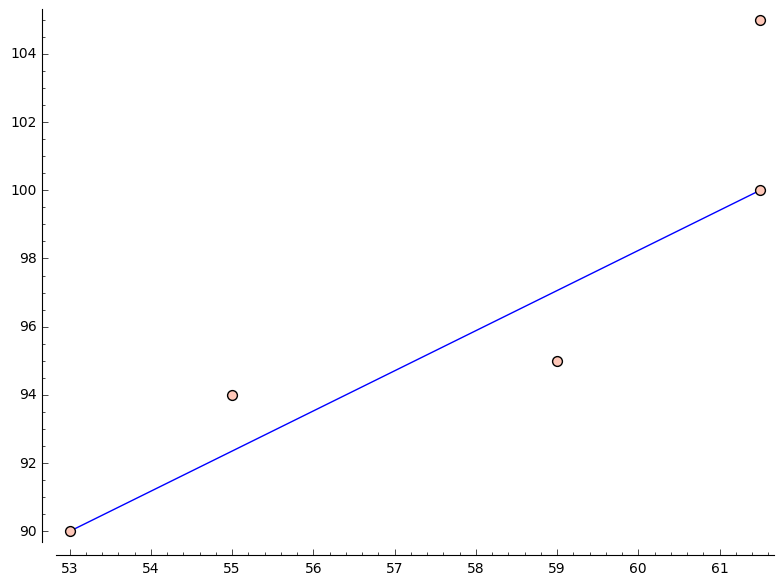
\includegraphics[scale=.5]{Figures/03_1.png}
        \end{center}

    \pagebreak
    \item % #3 Done
        Suppose you are preparing a schedule for classes.
        You have fixed number of classes and students.
        Every student told you which classes (s)he wants to attend.
        However, you do not have enough time slots to run all classes
        sequentially so you need to make some classes run in parallel.
        Create a schedule and argue why it is the best schedule in the sense
        that people as few conflicts as possible.
        You should be able to justify the optimality of the schedule in some sense.
        Make schedule with 3 and with 4 timeslots.
        Assume that there is no limit on how many classes can run in one timeslot.

        Use the following data
        {
        \tiny
            \begin{verbatim}
                [[0,0,0,1,0,1,0,1,0,0,1,0,1,0,0,1,1,1,1,1,1,1,1,0,1,1,1,1,0,0,1,0,0,0,1,1,1,1,1,1,0,1,1,1,1,1,1,0,0,1,0,1,0,0],
                [1,1,1,1,0,1,0,1,0,0,0,1,1,1,0,0,0,0,0,0,1,0,1,0,0,0,0,0,1,1,0,1,0,0,1,0,0,0,1,0,1,0,1,0,0,0,0,1,0,0,1,1,1,0],
                [1,0,1,0,1,0,1,0,1,1,1,1,0,0,1,1,1,1,1,1,0,0,0,1,1,1,0,1,0,0,0,1,0,0,1,1,0,1,1,1,0,1,1,1,1,1,0,0,0,1,1,0,0,0],
                [0,0,1,0,0,0,1,0,0,1,1,0,0,0,0,1,0,0,0,0,0,0,0,0,1,1,0,0,0,1,0,0,1,0,0,0,1,0,0,0,0,0,0,0,1,1,1,0,1,1,0,0,0,0],
                [1,0,0,1,0,1,0,0,0,1,0,0,1,0,0,0,0,0,0,0,0,1,0,1,0,0,1,0,1,0,1,1,0,1,0,0,0,0,0,0,0,0,0,0,0,0,0,0,1,0,0,0,1,0],
                [0,1,1,1,1,0,0,0,1,1,1,1,1,0,1,0,1,1,0,1,0,0,0,0,0,1,0,0,0,1,1,0,0,1,1,0,1,1,1,1,0,0,0,1,1,1,1,0,0,1,0,1,0,1],
                [0,0,1,1,0,1,1,0,0,1,1,1,0,1,1,0,1,1,0,1,0,1,1,0,0,1,1,0,0,0,1,0,0,0,0,0,0,1,0,0,0,0,1,1,0,1,1,0,0,1,0,1,1,0],
                [1,0,0,0,0,1,1,0,1,0,0,0,0,0,0,0,0,0,1,0,1,0,0,0,0,0,1,1,0,0,0,1,0,0,0,1,0,0,0,0,0,0,1,0,1,0,1,0,1,0,0,0,0,0],
                [0,1,0,0,0,1,1,0,1,0,1,0,0,0,0,1,1,1,0,1,0,1,1,1,1,1,0,0,0,0,1,0,1,0,0,0,1,0,1,1,0,0,1,1,1,0,1,0,0,0,0,1,0,1],
                [1,1,1,1,0,1,0,1,0,0,0,1,1,1,0,0,0,0,0,0,1,0,1,0,0,0,0,0,1,1,0,1,0,0,1,0,0,0,1,0,1,0,1,0,0,0,0,1,0,0,1,1,1,0],
                [1,0,1,0,1,0,1,0,1,1,1,1,0,0,1,1,1,1,1,1,0,0,0,0,1,1,0,1,0,0,0,1,0,0,1,1,0,1,1,1,0,1,1,1,1,1,0,0,0,1,1,0,0,0],
                [0,0,1,0,0,0,1,0,0,1,1,0,0,0,0,1,0,0,0,0,0,0,0,0,1,0,0,0,0,0,0,0,0,0,0,0,1,0,0,0,0,0,0,0,1,1,1,0,1,1,0,0,0,0],
                [1,0,0,1,0,1,0,0,0,1,0,0,1,0,0,0,0,0,0,0,0,1,0,0,0,0,1,0,1,0,1,1,1,0,0,0,0,0,0,0,0,0,0,0,0,0,0,0,1,0,0,0,1,0]]
            \end{verbatim}
        }
        Rows corresponds to one class, columns corresponds to one students.
        1 means the student wants to attend the class.

        Depending on the number of timeslots and the number of classes a
        student wants to take there is a maximum number of classes that a
        student can actually attend.
        For example if there are 4 timeslots and the student wants to take 7
        classes the maximum number of classes that they can take is 4.
        If there is a class that this student wants to take in all 4 timeslots
        then there really isn't any conflict, because the student can fill up
        their schedule with classes.
        On the other hand if there are 4 timeslots and the student only wants to
        take 2 different classes, then the maximum number of classes that the
        student can take is 2.

        This observation leads me to take the approach of maximizing the number
        of timeslots that a student can take a class they are interested in for
        each student.
        In order to do this I will introduce some notation.
        Let $s_{ij} = 1$ if student $j$ wants to take class $i$ and $s_{ij} = 0$
        if student $j$ does not want to take class $i$.
        Thus $s_{ij}$ is the $ij$ entry of the given data.
        Let $c_{ij}$ be a binary variables, where $c_{ij} = 1$ if class $i$ is
        scheduled for timeslot $j$, and $c_{ij} = 0$ otherwise.
        Let $w_{ij}$ be a binary variable, where $w_{ij} = 1$ if student $i$
        wants to take a class offered in timeslot $j$.
        Otherwise $w_{ij} = 0$, if there is no class in timeslot $j$ that
        student $i$ wants to take.
        Lastly let $n_t$ be the number of timeslots, $n_c$ be the number of
        classes, and $n_s$ be the number of students.
        Since we are using binary variables, this implies the linear program
        will in fact be an integer linear program.

        Thus the objective function of our linear program will be maximizing
        \[
            \sum*{i = 1}{n_s}{\sum*{j=1}{n_t}{w_{ij}}}.
        \]
        This double sum is the total number of class periods for all students
        which contains a class that they want to take.

        The following constraints are also necessary.
        First every class can only be schedule once, so
        \[
            \sum{j=1}{n_t}{c_{ij}} = 1
        \]
        This means that each class can only be in one timeslot.

        We also need constraints to enforce the definition of the binary
        variables $w_{ij}$.
        In other words the variables $w_{ij}$ depends on the variables
        $c_{ij}$.
        Let $n_{ij}$ be the total number of classes student $i$ is interested in
        taking during timeslot $j$.
        This can be calculated as
        \[
            n_{ij} = \sum{k = 1}{n_c}{s_{ki} c_{kj}}
        \]
        If $n_{ij} \ge 1$, then $w_{ij} = 1$.
        The constraint
        \[
            n_{ij} \le M w_{ij}
        \]
        enforces this when $M$ is sufficiently large.
        This works because $w_{ij}$ is binary and can only be $0$ or $1$, so if
        $n_{ij} > 0$, then $w_{ij} > 0$ which implies $w_{ij} = 1$.
        In this problem $M$ being sufficiently large means that $M$ must be
        larger than the largest possible value of $n_{ij}$, which in this case
        means that $M > n_c$.

        If on the other hand $n_{ij} = 0$, then $w_{ij} = 0$.
        The constraint
        \[
            n_{ij} \ge w_{ij}
        \]
        enforces this condition.
        If $n_{ij} = 0$, then $w_{ij} \neq 1$ as $0 \ngeq 1$, so $w_{ij} = 0$.
        This also dosn't contradict the previous constraint as if $n_{ij} = 1$,
        then $n_{ij} = 1 \ge 1 = w_{ij}$.

        Thus the full integer linear program is
        \[
            \begin{array}{ll@{}ll}
                \max* & \sum*{i = 1}{n_s}{\sum*{j=1}{n_t}{w_{ij}}} \\
                \text{s.t.} & \sum{j=1}{n_t}{c_{ij}} = 1 \hskip 1em &1 \le i \le n_c \\
                            & n_{ij} \le M w_{ij}         &1 \le i \le n_s \hskip 1em 1 \le j \le n_t\\
                            & n_{ij} \ge w_{ij}           &1 \le i \le n_s \hskip 1em 1 \le j \le n_t \\
                            & 0 \le c_{ij} \le 1          &1 \le i \le n_c \hskip 1em 1 \le j \le n_t \\
                            & 0 \le w_{ij} \le 1          &1 \le i \le n_s \hskip 1em 1 \le j \le n_t \\
                            & c_{ij} \in \ZZ              &1 \le i \le n_c \hskip 1em 1 \le j \le n_t \\
                            & w_{ij} \in \ZZ              &1 \le i \le n_s \hskip 1em 1 \le j \le n_t
            \end{array}
        \]

        The following sage script implements this integer linear program.
        \lstinputlisting[language=Sage, firstline=17]{03_3.sage}
        Importing the given data as matrix $s$ is not shown.
        As described at the beginning of the problem there is a maximum number
        of classes that can be taken depending on the number of timeslots.
        This is shown as part of the output.

        Running this script with 3 timeslots results in
        \begin{verbatim}
            157 out of 158
            1: Class 3, Class 8, Class 9, Class 10
            2: Class 2, Class 4, Class 5, Class 11, Class 12
            3: Class 1, Class 6, Class 7, Class 13
        \end{verbatim}

        With 4 timeslots
        \begin{verbatim}
            194 out of 202
            1: Class 2, Class 7, Class 8, Class 12
            2: Class 5, Class 9, Class 11
            3: Class 1, Class 6, Class 13
            4: Class 3, Class 4, Class 10
        \end{verbatim}

\end{enumerate}
\end{document}
